\chapter{Addressing Scheme}
\section{Scheme}
\begin{figure}[H]
    \centering
    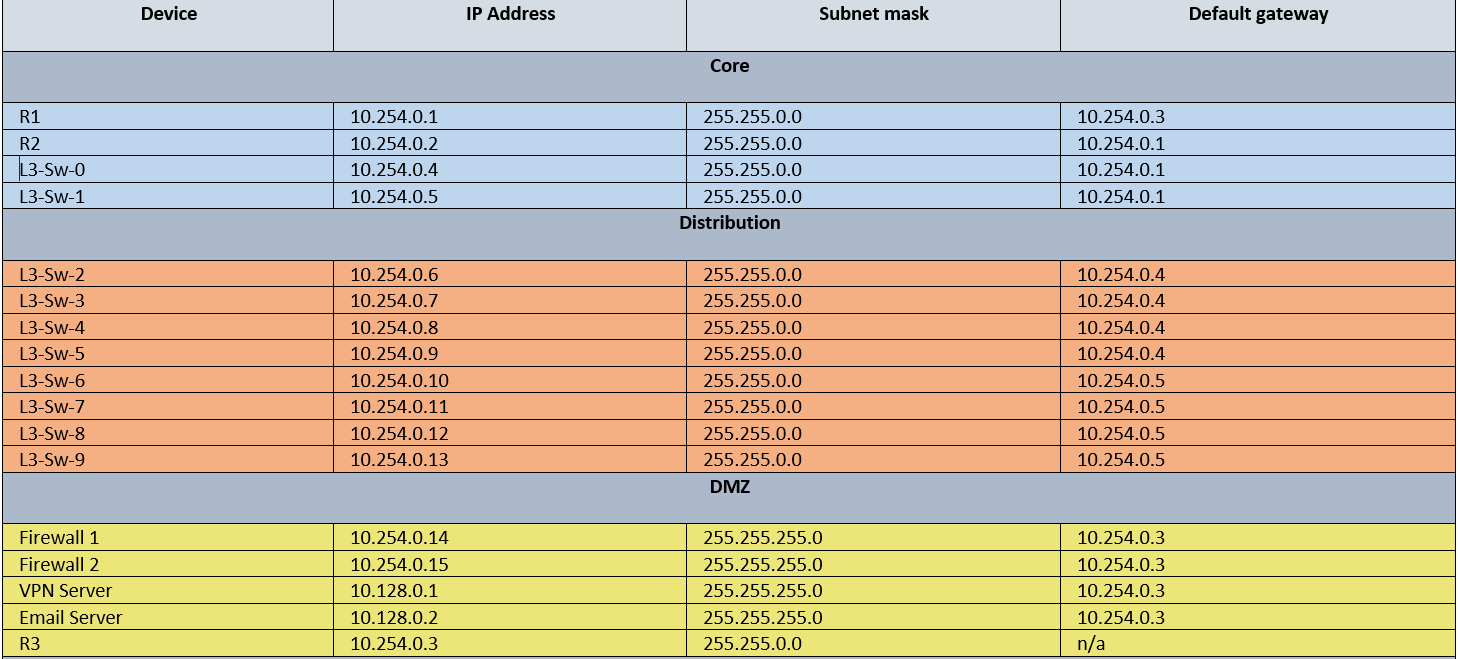
\includegraphics[width=15cm]{Figures/scheme_1.png}
    \caption{Core layer, distribution layer and DMZ addressing scheme.}
\end{figure}
\begin{figure}[H]
    \centering
    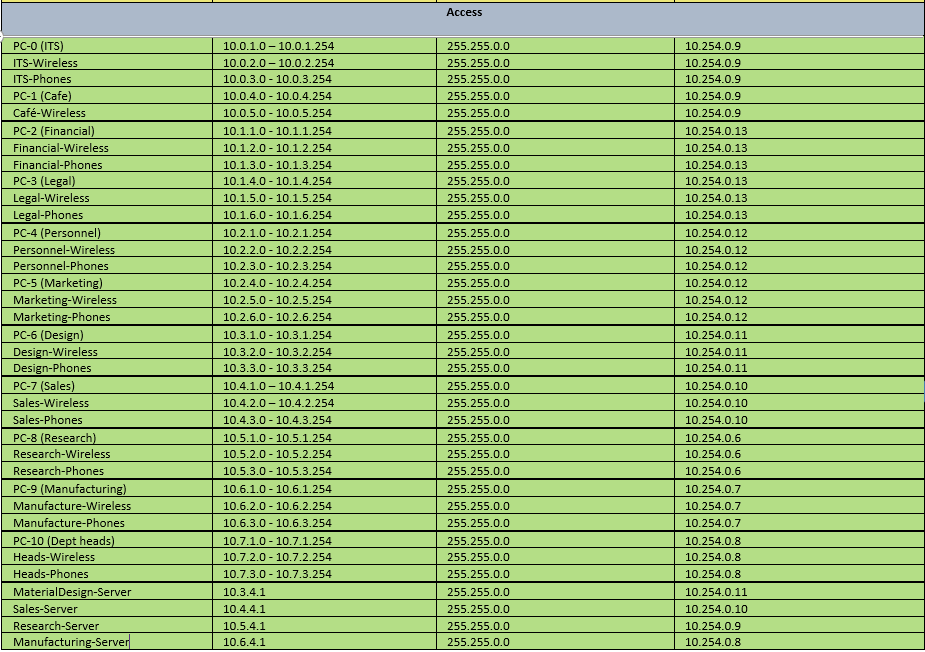
\includegraphics[width=15cm]{Figures/scheme_2.png}
    \caption{Access layer addressing scheme.}
\end{figure}
\section{Justifications}
\subsection{Private addressing}
Due to using the private addressing scheme that is discussed within the appendices, we are able to subnet and address the network to fit a hierarchical model. The addresses are designated via; 10.x.y.z WHERE x=floor, y=department, z=end device. We can be wasteful and have a lot of room for adding new devices in case of expansion of the company.
\subsection{Address ranges}
The address ranges used are designed to correlate with the department's location within the logical and physical location of their respective devices within the network. Department servers are located within their required subnets and accessible to those who have the authentication. The DMZ and core of the network have been given their own subnets in order to keep them secure.
\subsection{Access}
The server room will be the primary aspect of our network access, each department will need to have access to their servers and remote employee's must also be able to access components from outside the network. The router R1 has the capability of performing NAT/PAT which has allowed us to use the addressing scheme we have in place.
\subsection{Layer 3 devices}
The layer 3 switches included within the distribution layer are capable of routing the traffic between the different segments of the network, and will be able to enforce traffic rules which will provide access and security for each part of the network.